% this is a template for papers or notes written in Chinese
\documentclass[a4paper]{article}

\usepackage[
    fontset=none,%设置中文支持,并自定义字体
    zihao=5,%默认字号为五号
    heading=true,%允许后续自定义标题样式
    scheme=chinese,%自动将文档样式中文化,例如图标标题
    punct=quanjiao,%全角式标点符号
    space=auto,%中文后接换行不会添加空格,但是英文会添加空格,需要用%手动取消
    linespread=1.3,%行距倍数是1.3
    autoindent=true,%自动缩进两个中文宽度
    ]{ctex}
\ctexset{
    % tday=small,%小写样式的日期
    contentsname={目录},
    listfigurename={插图},
    listtablename={表格},
    figurename={图},
    tablename={表},
    abstractname={摘要},
    indexname={索引},
    appendixname={附录},
    bibname={参考文献},
    proofname={证明},
    % refname={参考文献},%只适用于beamer
    % algorithmname={算法},
    % continuation={(续)},%beamer续页的标识
    section={
        format+ = \Large\heiti\raggedright,
        name = {,\num\textbf{.}\hspace{1ex}},
        number={\num\thesection},
        nameformat={},
        numberformat={},
        aftername={},
        titleformat={},
        aftertitle={},
        runin=false,%对section级以下有用,标题是否和正文在同一段上
        beforeskip={3.5ex plus 1ex minus .2ex},%标题前垂直间距
        afterskip={2.3ex plus .2ex}%标题后垂直间距
    },
    subsection={
        format+ = \large\heiti\raggedright,
        name = {,\num\textbf{.}\hspace{1ex}},
        number={\num\thesubsection},
        nameformat={},
        numberformat={},
        aftername={},
        titleformat={},
        aftertitle={},
        runin=false,%对section级以下有用,标题是否和正文在同一段上
        beforeskip={3.5ex plus 1ex minus .2ex},%标题前垂直间距
        afterskip={2.3ex plus .2ex}%标题后垂直间距
    },
    subsubsection={
        format+ = \normalsize\heiti\raggedright,
        name = {,\num\textbf{.}\hspace{1ex}},
        number={\num\thesubsubsection},
        nameformat={},
        numberformat={},
        aftername={},
        titleformat={},
        aftertitle={},
        runin=false,%对section级以下有用,标题是否和正文在同一段上
        beforeskip={3.5ex plus 1ex minus .2ex},%标题前垂直间距
        afterskip={2.3ex plus .2ex}%标题后垂直间距
    },
    }

% 中文默认字体: 思源宋体,粗体为思源宋体半粗体,斜体为方正楷体_GBK
\setCJKmainfont{Source Han Serif SC}[BoldFont={Source Han Serif SC Heavy}, ItalicFont=FZKai-Z03S]
% 中文无衬线字体:思源黑体,粗体为思源黑体粗体
\setCJKsansfont{Source Han Sans CN}[BoldFont={Source Han Sans CN Heavy}]
% 中文等宽字体:微软雅黑light
\setCJKmonofont{Microsoft YaHei}[ItalicFont={Microsoft YaHei Light}]

\newCJKfontfamily\songti{Source Han Serif SC}[BoldFont={Source Han Serif SC Heavy}]
\newCJKfontfamily\xbsong{Source Han Serif SC SemiBold} % 小标宋
\newCJKfontfamily\dbsong{Source Han Serif SC Bold} % 大标宋
\newCJKfontfamily\cusong{Source Han Serif SC Heavy} % 粗宋
\newCJKfontfamily\heiti{Source Han Sans CN}[BoldFont={Source Han Sans CN Heavy}]
\newCJKfontfamily\dahei{Source Han Sans CN Medium} % 大黑
\newCJKfontfamily\cuhei{Source Han Sans CN Heavy} % 粗黑
\newCJKfontfamily\fangsong{FZFangSong-Z02S}
\newCJKfontfamily\kaiti{FZKai-Z03S}[ItalicFont={Microsoft YaHei Light}]%这个斜体只是用于lstlisting环境中的中文注释
% \newCJKfontfamily\kaiti{FZKai-Z03S}[ItalicFont={FZZJ-LZXTFSJW}]%这个斜体只是用于lstlisting环境中的中文注释
\setsansfont{Arial}
\setmonofont{Consolas}%设置西文等宽字体
\newfontfamily\code{Consolas}
\newfontfamily\num{Arial}

\usepackage{geometry}%设置整体页面布局
\geometry{a4paper}
\geometry{left=2cm,right=2cm,top=2.54cm,bottom=2.54cm}%word常规页边距
% \geometry{left=1.27cm,right=1.27cm,top=1.27cm,bottom=1.27cm}%word窄页边距
\setlength{\headheight}{13pt}%避免warning


\usepackage{fancyhdr}%必须在geometry包之后使用
\fancyhf{}
\makeatletter
\lhead{{\dahei \@title}}%可以使用thepage,CTEXthechapter,CTEXthesection
\makeatother
\rhead{\textbf{\num- \thepage{} -}}
\renewcommand\headrulewidth{1.5pt}%设置眉头宽度
\pagestyle{fancy}

\usepackage[ruled,algosection,lined,longend,fillcomment,linesnumbered,resetcount,titlenotnumbered]{algorithm2e}
%参数解释:带框,按section编码,有竖线,end前带if等关键词,注释占满整行,代码部分编号(不包括输入输出、注释),每个代码块重新编号,可以调用TitleOfAlgo来打印算法标题但不作为单独的算法编码
%附带algorithm,function,procedure环境,其中function,procedure环境下,设置caption时,必须带有(),
%()之前的字符会被视为宏,可以在接下来的部分用\名字()来调用,所以推荐辅助函数用function,其中的某些展开部分用procedure,描述算法整体使用algorithm
\DontPrintSemicolon
\SetAlCapSkip{2ex}
\SetSideCommentRight
\SetFillComment
\newcommand{\forcond}{$i=0$ \KwTo $n$}
\SetKw{downto}{downto}%自定义关键词
\SetKwFunction{funcmacro}{text}%自定义函数名,实际上function环境是在定义宏的同时说明了其内容
\SetKwProg{procedmacro}{text}{begin text}{end text}%自定义步骤,和function类似,但是后面两个参数可以设置开始和结尾的标志,和if等环境一样
\SetKwData{datamacro}{text}%可以用于突出特殊的变量,例如数据结构
\SetKwFunction{FRecurs}{FnRecursive}
\SetKwProg{Fn}{Function}{begin}{end}

\usepackage[strict]{changepage}
\usepackage{framed}%色块支持
\definecolor{formalshade}{rgb}{0.95,0.95,1} % 文本框颜色
% ------------------******-------------------
% 注意行末需要把空格注释掉,不然画出来的方框会有空白竖线
\newenvironment{formal}{%
\def\FrameCommand{%
\hspace{1pt}%
{\color{DarkBlue}\vrule width 2pt}%
{\color{formalshade}\vrule width 4pt}%
\colorbox{formalshade}%
}%
\MakeFramed{\advance\hsize-\width\FrameRestore}%
\noindent\hspace{-4.55pt}% disable indenting first paragraph
\begin{adjustwidth}{}{7pt}%
\vspace{2pt}\vspace{2pt}%
}
{%
\vspace{2pt}\end{adjustwidth}\endMakeFramed%
}

% 自定义标题格式
\makeatletter
\renewcommand{\maketitle}{
  \begin{center}
    \thispagestyle{fancy}
    {\quad}\\
    \vspace{0.1\textheight}
    {\huge\sffamily\bfseries\@title}\\ % 标题字体大小、粗体、颜色
    \vspace{2em} % 标题与作者名之间的垂直空间
    {\large\sffamily\@author} \\
  \end{center}
}
\makeatother

\usepackage{graphicx}

\title{作业{\hspace{1ex}}HW6{\hspace{1ex}}实验报告}
\author{姓名:范潇{\quad}学号:2254298{\quad}日期:\today}
\date{}
\begin{document}
\maketitle
% \thispagestyle{fancy}%用于单独设置某页的样式,此处用于设置标题页的格式
\section{涉及数据结构和相关背景}

\newpage
\section{实验内容}
\section{题目一}
\subsection{实验目的}
安装配置UNIX V6++的运行环境。
\subsection{实验内容}
\begin{enumerate}
    \item 安装后端服务根证书;
    \item 登录实验平台;
    \item  运行远程桌面环境;
    \item 初始化代码仓库;
    \item 启动UNIX V6++运行环境。
\end{enumerate}
\subsection{实验过程}
安装完后端服务根证书后,登录网站http://vesper-system.pages.tongji.edu.cn/vesper-front/,然后如图\ref{changeCode}所示,修改密码。接着,如图
\ref{changeName}所示,修改主机名。之后,我在GitLab中创建了自己的代码分支。等待桌面环境启用后,如图\ref{genCode}所示,生成密钥,然后如图\ref{setCode}所示,将公钥上传至GitLab。
当我尝试下载实验工具包时,要求我输入用户名和密码,为此,为如图\ref{setToken}所示,申请了个人访问令牌用作密码。下载完成后,将工作目录设置为unix-v6pp-tongji,然后如图\ref{init},\ref{makeQemu},\ref{qemu}所示,依次执行init.sh和make qemu命令,
最终启动了UNIX V6++界面并如图\ref{helloWorld}所示,执行了echo命令。

\begin{figure}[!htbp]
    \centering
    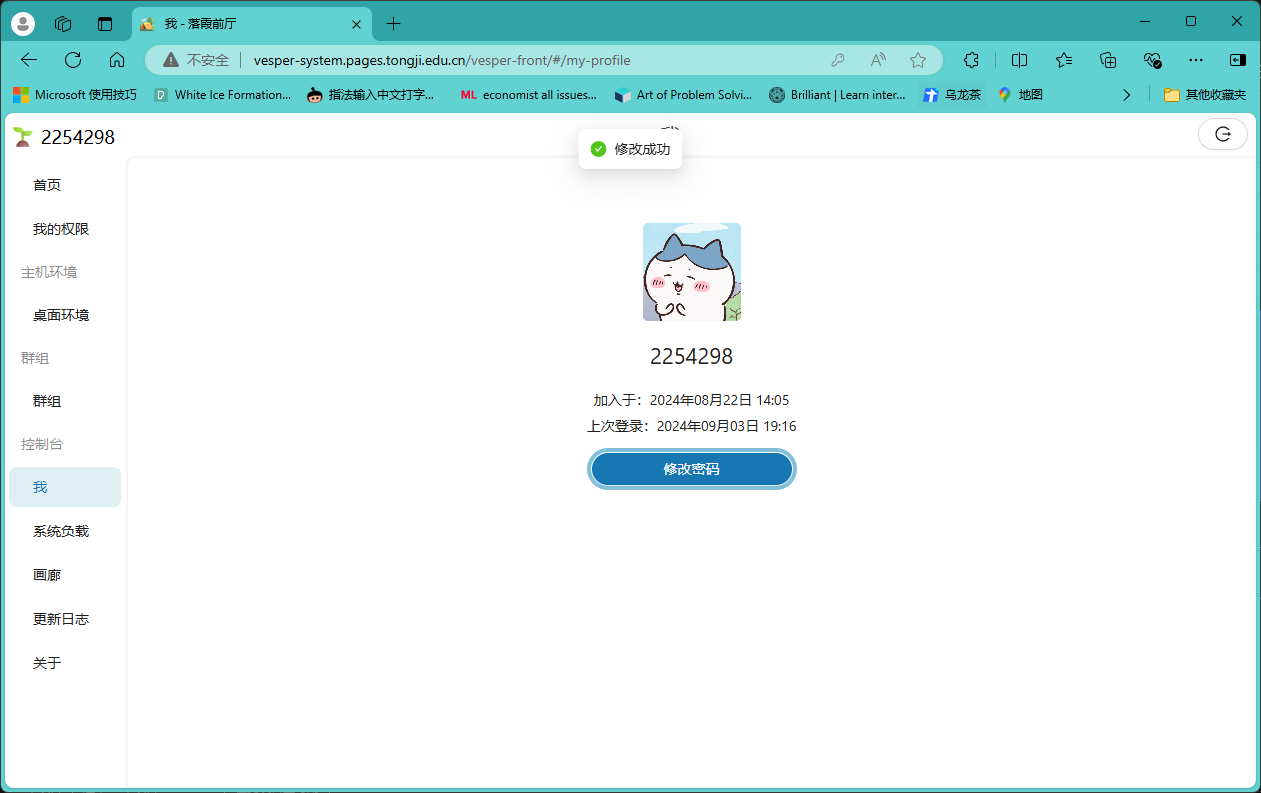
\includegraphics[scale=0.4]{fig/changeCode.png}
    \caption{修改密码}\label{changeCode}
\end{figure}
\begin{figure}[!htbp]
    \centering
    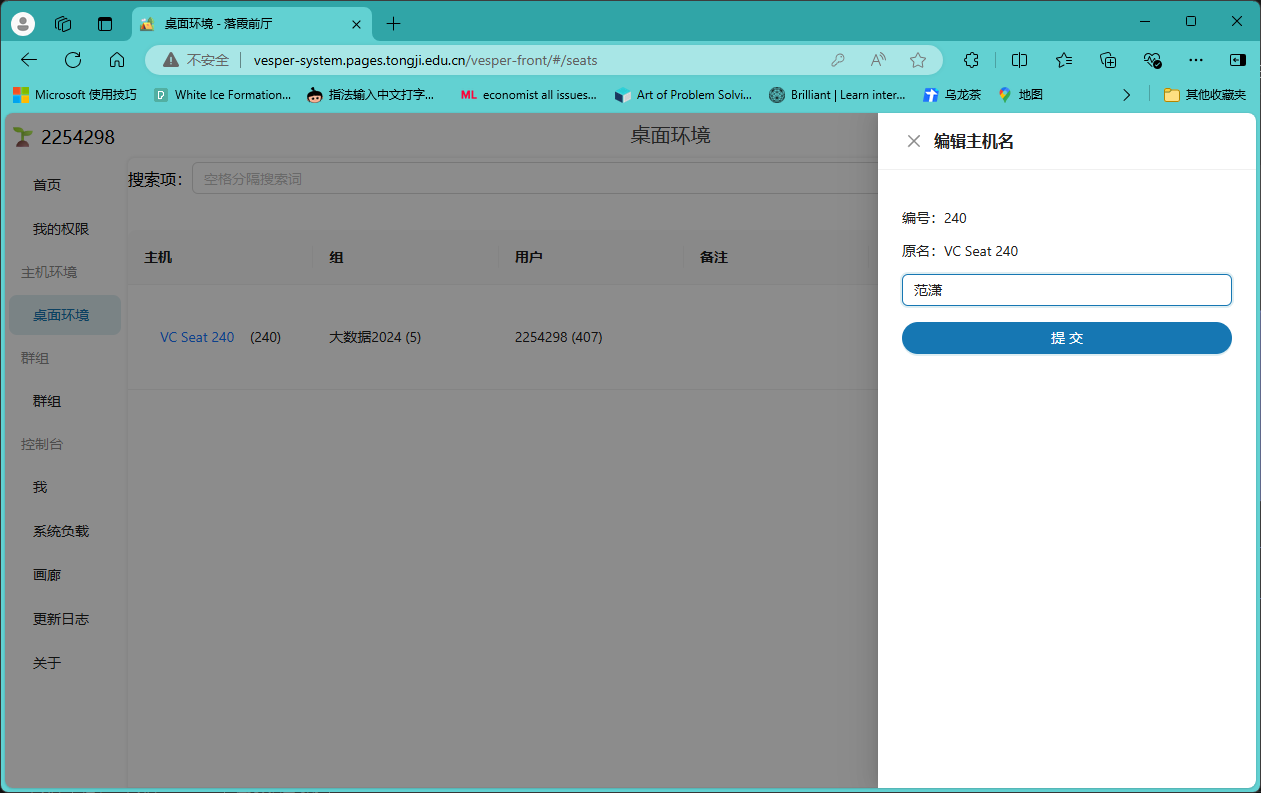
\includegraphics[scale=0.4]{fig/changeName.png}
    \caption{修改主机名}\label{changeName}
\end{figure}

\begin{figure}[!htbp]
    \centering
    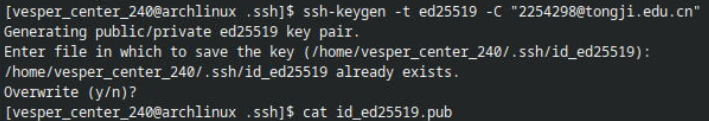
\includegraphics[scale=0.7]{fig/genCode.png}
    \caption{生成密钥}\label{genCode}
\end{figure}

\begin{figure}[!htbp]
    \centering
    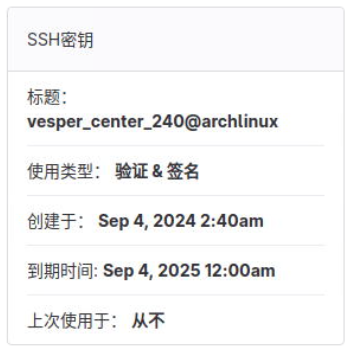
\includegraphics[scale=1]{fig/setCode.png}
    \caption{在GitLab中上传公钥}\label{setCode}
\end{figure}

\begin{figure}[!htbp]
    \centering
    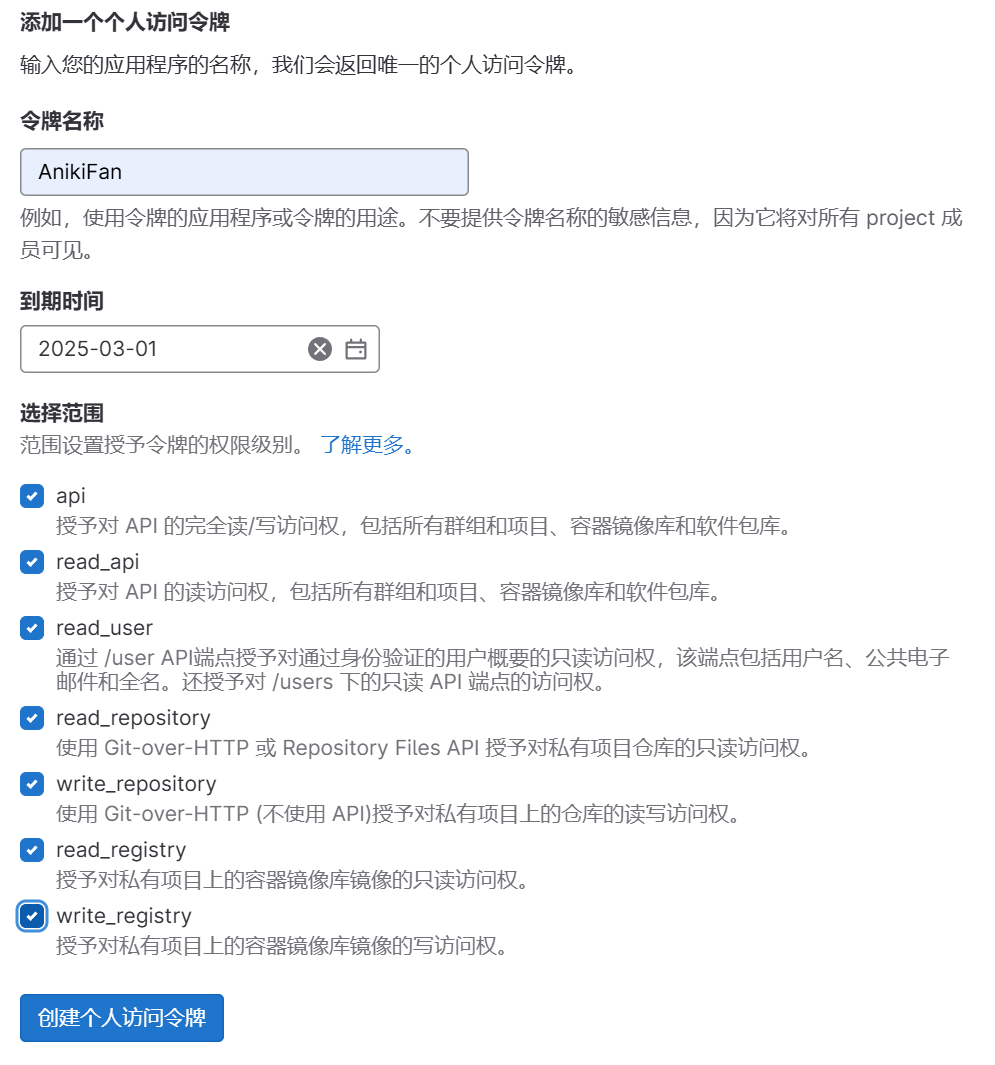
\includegraphics[scale=0.4]{fig/setToken.png}
    \caption{设置个人访问令牌}\label{setToken}
\end{figure}

\begin{figure}[!htbp]
    \centering
    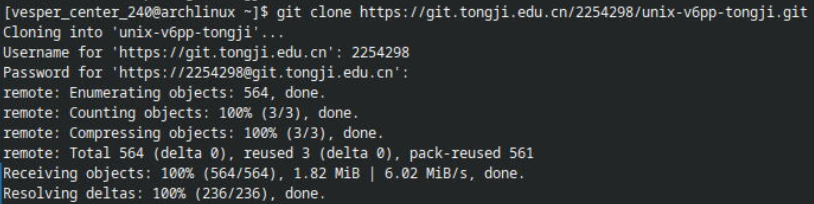
\includegraphics[scale=0.4]{fig/downloadTool.png}
    \caption{下载实验工具包}\label{downloadTool}
\end{figure}

\begin{figure}[!htbp]
    \centering
    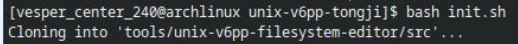
\includegraphics[scale=1]{fig/init.png}
    \caption{执行init.sh}\label{init}
\end{figure}

\begin{figure}[!htbp]
    \centering
    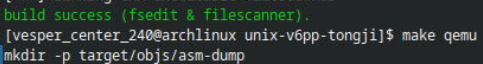
\includegraphics[scale=1]{fig/makeQemu.png}
    \caption{执行make qemu}\label{makeQemu}
\end{figure}

\begin{figure}[!htbp]
    \centering
    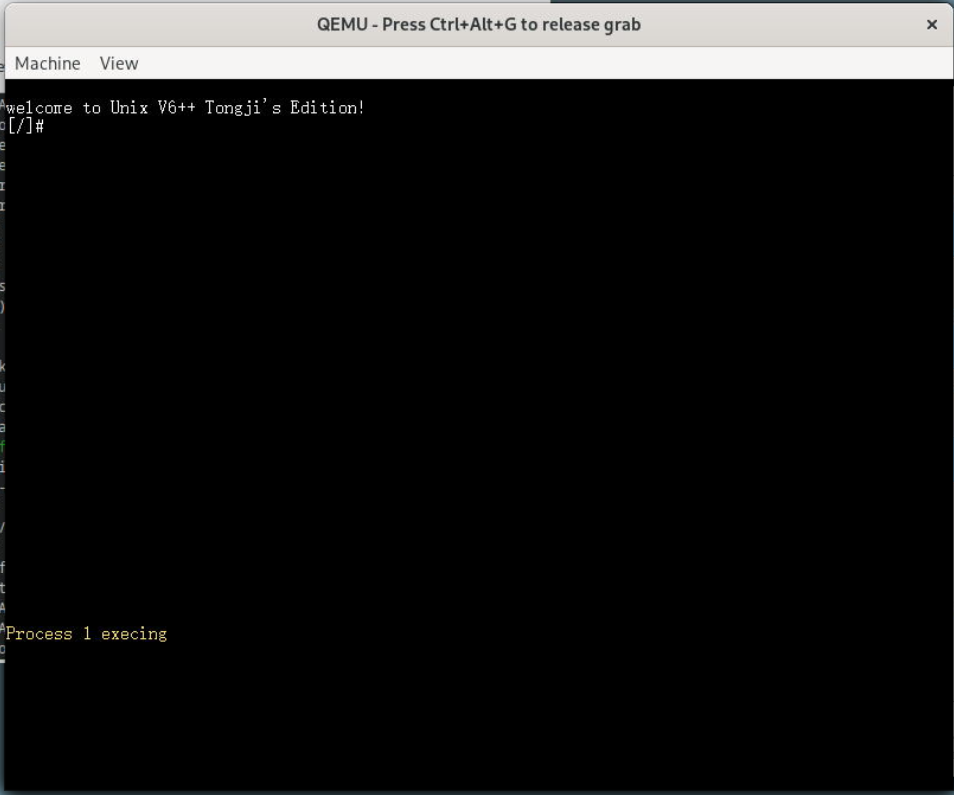
\includegraphics[scale=0.5]{fig/qemu.png}
    \caption{UNIX V6++界面}\label{qemu}
\end{figure}

\begin{figure}[!htbp]
    \centering
    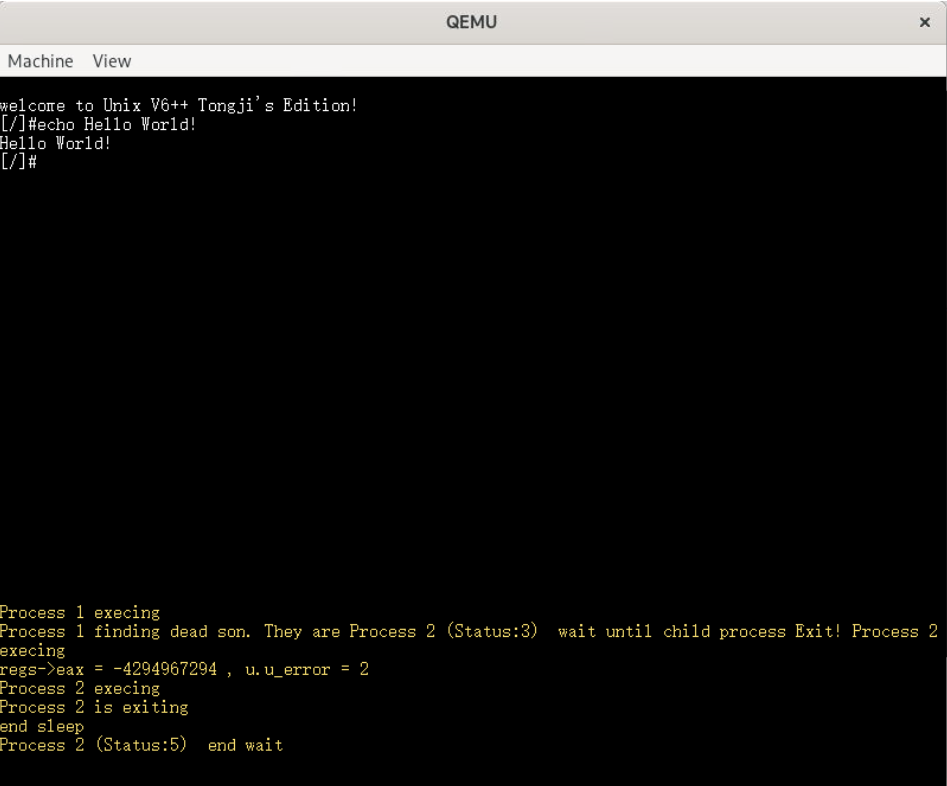
\includegraphics[scale=0.5]{fig/helloWorld.png}
    \caption{执行echo命令}\label{helloWorld}
\end{figure}

\newpage
\subsection{求逆序对数}
\begin{formal}
    {\cuhei 问题描述:}
请求出整数序列$A$的所有逆序对个数。
\end{formal}
\begin{formal}
    {\cuhei 输入要求:}

    输入包含多组测试数据,每组测试数据有两行。
第一行为整数$N(1 \leq N \leq 20000)$,当输入0时结束;
第二行为$N$个整数,表示长为$N$的整数序列。
\end{formal}
\begin{formal}
    {\cuhei 输出要求:}

    每组数据对应一行,输出逆序对的个数。
\end{formal}
\subsubsection{数据结构设计}
\begin{lstlisting}[name=Q1]
typedef struct {
    int data[MAXN] ;//整数序列
    int length ;//整数序列长度
}array ;
\end{lstlisting}
\subsubsection{功能描述}

% 在直接插入排序中,一次位置调整便能消去一对逆序对,而当排序结束时,逆序对数为零。
% 逆序对数等于直接插入排序中位置交换的次数。为了降低时间复杂度,使用折半插入排序,并
% 直接利用插入位置计算出交换次数。
% \begin{procedure}
%     \tcp*[h]{A为给定整数序列,i为待排序元素下标}\;
%     \tcp*[h]{返回待插入位置}\;
%     l = 0\;
%     h = i-1\;
%     \While(\tcp*[h]{确保mid+1合法}){l<h}
%     {
%         mid = $\lfloor$(l+h)/2$\rfloor$\;
%         \lIf(\tcp*[h]{确保稳定性}){A.data[mid]$\leq$A.data[i]<A.data[mid+1]}{\KwRet{mid+1}}
%         \leIf{A.data[mid]>A.data[i]}{h=mid}{l=mid+1}
%     }
%     \leIf{A.data[l]$\leq$A.data[i]}{\KwRet{l+1}}{\KwRet{l}}
%     \caption{BinarySearch(A,i)}
% \end{procedure}
% \begin{algorithm}
%     \tcp*[h]{A为给定整数序列}\;
%     \For{j = 2 \KwTo A.length}
%     {
%         key = A.data[j]\;
%         dest = \BinarySearch(A,j)\;
%         \For{i = j-1 \downto dest}
%         {
%             A.data[i + 1] = A.data[i]\;
%             i = i - 1\;
%         }
%         A.data[dest] = key\;
%         A.counter = A.counter + j - dest\;
%     }
%     \KwRet{A.counter}
%     \caption{Count-Inversion}
% \end{algorithm}

\begin{function}[H]
    mid = $\lfloor$(r+l)/2$\rfloor$\;
    $n_1$ = mid - l + 1 \;
    $n_2$ = r - mid\;
    创建大小分别为 $n_1,n_2$的数组 $L,R$\;
    \lFor{i=0 \KwTo $n_1$-1}{L[i]=A[l+i]}
    \lFor{i=0 \KwTo $n_2$-1}{R[i]=A[mid+1+i]}
    m = 0\;
    n = 0\;
    counter = 0\;
    \For(\tcp*[h]{合并子序列}){i=0 \KwTo $n_1+n_2-1$}
    {
        \eIf{(L[m] $\leq$R[n] and m <$n_1$) or (n $\geq n_2$)}
        {
            A[l+i] = L[m]\;
            m = m + 1\;
        }
        {
            A[l+i] = R[n]\;
            counter = counter + $n_1$ + n - i\tcp*[h]{需要移动的“步数”}\;
            n = n + 1\;
        }
    }
    \KwRet{counter}
    \caption{Merge(A,r,l)}
\end{function}
\begin{function}
    \SetKwFunction{CountInversion}{CountInversion}
    \tcp*[h]{A为给定整数序列}\;
    \tcp*[h]{最终解答调用\CountInversion(A,0,A.length-1)}\;
    \lIf{r == l}{\KwRet{0}}
    mid = $\lfloor$(r+l)/2$\rfloor$\;
    \KwRet{\CountInversion(A,l,mid) + \CountInversion(A,mid+1,r) + \Merge(A,l,r)}\;
    \caption{CountInversion(A,r,l)}
\end{function}
\subsubsection{调试分析}
本题采用输出关键变量进行调试。选用的关键变量是\Merge()中涉及到的数组部分以及对应的\emph{counter}。

在调试的过程中,遇到了多次相同输入,但是输出不同的情况,因此判断是内存出现问题。查看数组部分的输出信息,
发现在运行过程中数组内部出现了异常元素。经过排查后发现是“合并子序列”步骤中,当一个子序列以及全部转移完毕时,
仍有可能继续转移,从而产生内存溢出,加上 $m<n_1,n\geq n_2$条件后便恢复正常。
\subsubsection{总结和体会}
我一开始使用折半插入排序,但是最终有两个样例由于超时而无法通过,这是因为折半插入排序移动元素的平均时间复杂度仍为 $O(n^2)$。
最后我在归并排序的基础上进行调整,时间复杂度维持在了 $\Theta(n\lg n)$。使用该方法时,我仍然有两个样例没有通过,原因是
内存使用过多,经过排查,是因为只申请了内存,而没有释放。在调试的过程中,我也体会到了处理边界情况的重要性,如果能够
合理设置哨兵,例如在数组 $L,R$结尾设置两个哨兵,便可以在保持程序简洁的同时确保正确性。
\newpage
\subsection{题目名称}
\begin{formal}
    {\cuhei 问题描述:}

    测试\\
    测试
\end{formal}
\begin{formal}
    {\cuhei 输入要求:}

    测试\\
    测试
\end{formal}
\begin{formal}
    {\cuhei 输出要求:}

    测试\\
    测试
\end{formal}
\subsubsection{数据结构设计}
\begin{lstlisting}[name=Q1]
//
test
test
\end{lstlisting}
\subsubsection{功能描述}
\begin{lstlisting}[name=F11]
//
test
test
\end{lstlisting}
\begin{function}
    \tcp*[h]{describe your function}\;
    \KwIn{input}
    \KwOut{output}
    \caption{NameOfFunction()}
\end{function}
\subsubsection{调试分析}
\subsubsection{总结和体会}
\newpage
\subsection{题目名称}
\begin{formal}
    {\cuhei 问题描述:}

    测试\\
    测试
\end{formal}
\begin{formal}
    {\cuhei 输入要求:}

    测试\\
    测试
\end{formal}
\begin{formal}
    {\cuhei 输出要求:}

    测试\\
    测试
\end{formal}
\subsubsection{数据结构设计}
\begin{lstlisting}[name=Q1]
//
test
test
\end{lstlisting}
\subsubsection{功能描述}
\begin{lstlisting}[name=F11]
//
test
test
\end{lstlisting}
\begin{function}
    \tcp*[h]{describe your function}\;
    \KwIn{input}
    \KwOut{output}
    \caption{NameOfFunction()}
\end{function}
\subsubsection{调试分析}
\subsubsection{总结和体会}
\newpage
\subsection{题目名称}
\begin{formal}
    {\cuhei 问题描述:}

    测试\\
    测试
\end{formal}
\begin{formal}
    {\cuhei 输入要求:}

    测试\\
    测试
\end{formal}
\begin{formal}
    {\cuhei 输出要求:}

    测试\\
    测试
\end{formal}
\subsubsection{数据结构设计}
\begin{lstlisting}[name=Q1]
//
test
test
\end{lstlisting}
\subsubsection{功能描述}
\begin{lstlisting}[name=F11]
//
test
test
\end{lstlisting}
\begin{function}
    \tcp*[h]{describe your function}\;
    \KwIn{input}
    \KwOut{output}
    \caption{NameOfFunction()}
\end{function}
\subsubsection{调试分析}
\subsubsection{总结和体会}
\newpage
\section{实验总结}
用于排序的各个算法各有特点,即使是高效排序算法,在处理极端和特殊情况时的表现差异也很明显。因此,在实际应用时,
需要结合对于输入数据的已有知识,选取最为合适的排序算法。同时,如果只是把排序作为其他算法中的子步骤,在保证时间复杂度
的前提下,可以考虑排序算法的稳定排序、部分排序等特性对于算法设计是否有用,从而选取最合适的排序算法。
\end{document}